\begin{figure*}
  \centering
  \begin{subfigure}[t]{0.6\textwidth}
    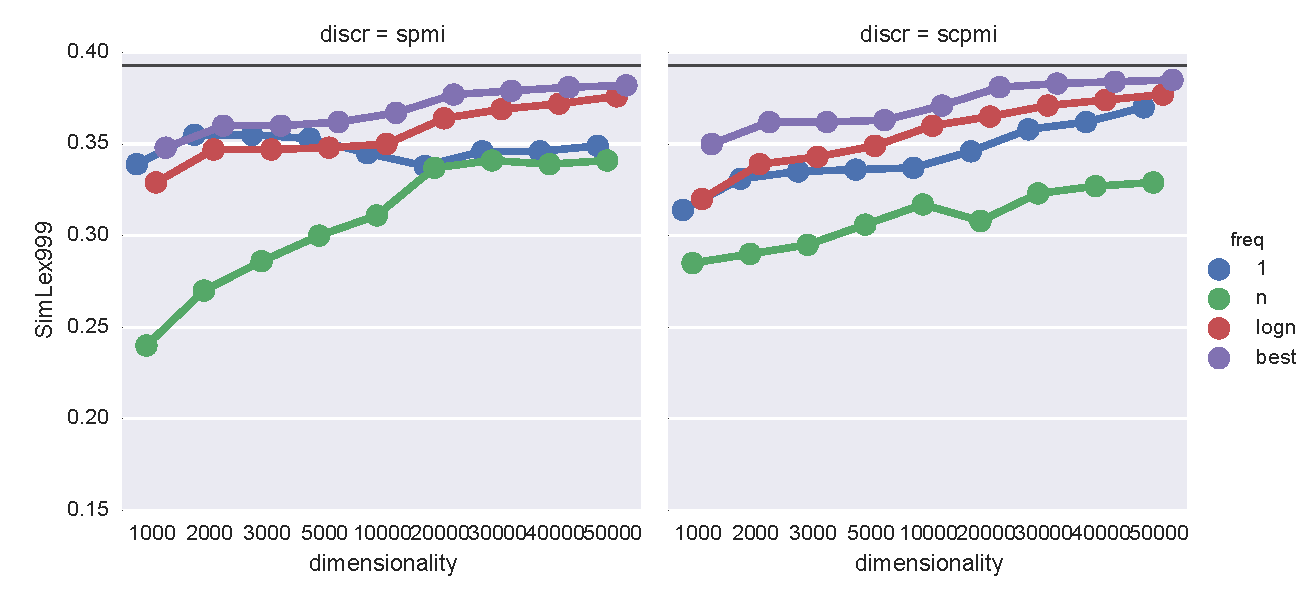
\includegraphics[width=\textwidth]{supplement/figures/SimLex999-best}
    \caption{\textbf{SimLex-999.} The black line refers to the score of 0.393. \\
      This work: 0.385,
      SGNS: 0.438,
      GloVe: 0.398.
    }
    \label{fig:best-simlex}
  \end{subfigure}
  ~
  \begin{subfigure}[t]{0.37\textwidth}
    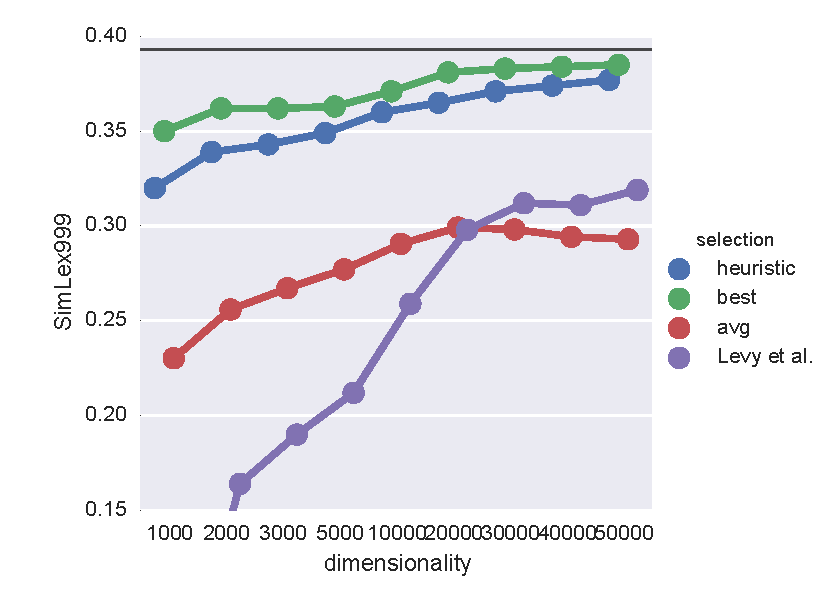
\includegraphics[width=\textwidth]{supplement/figures/SimLex999-global-best}
    \caption{\textbf{SimLex-999.}
    }
    \label{fig:global-best-simlex}
  \end{subfigure}

  \begin{subfigure}[t]{0.6\textwidth}
    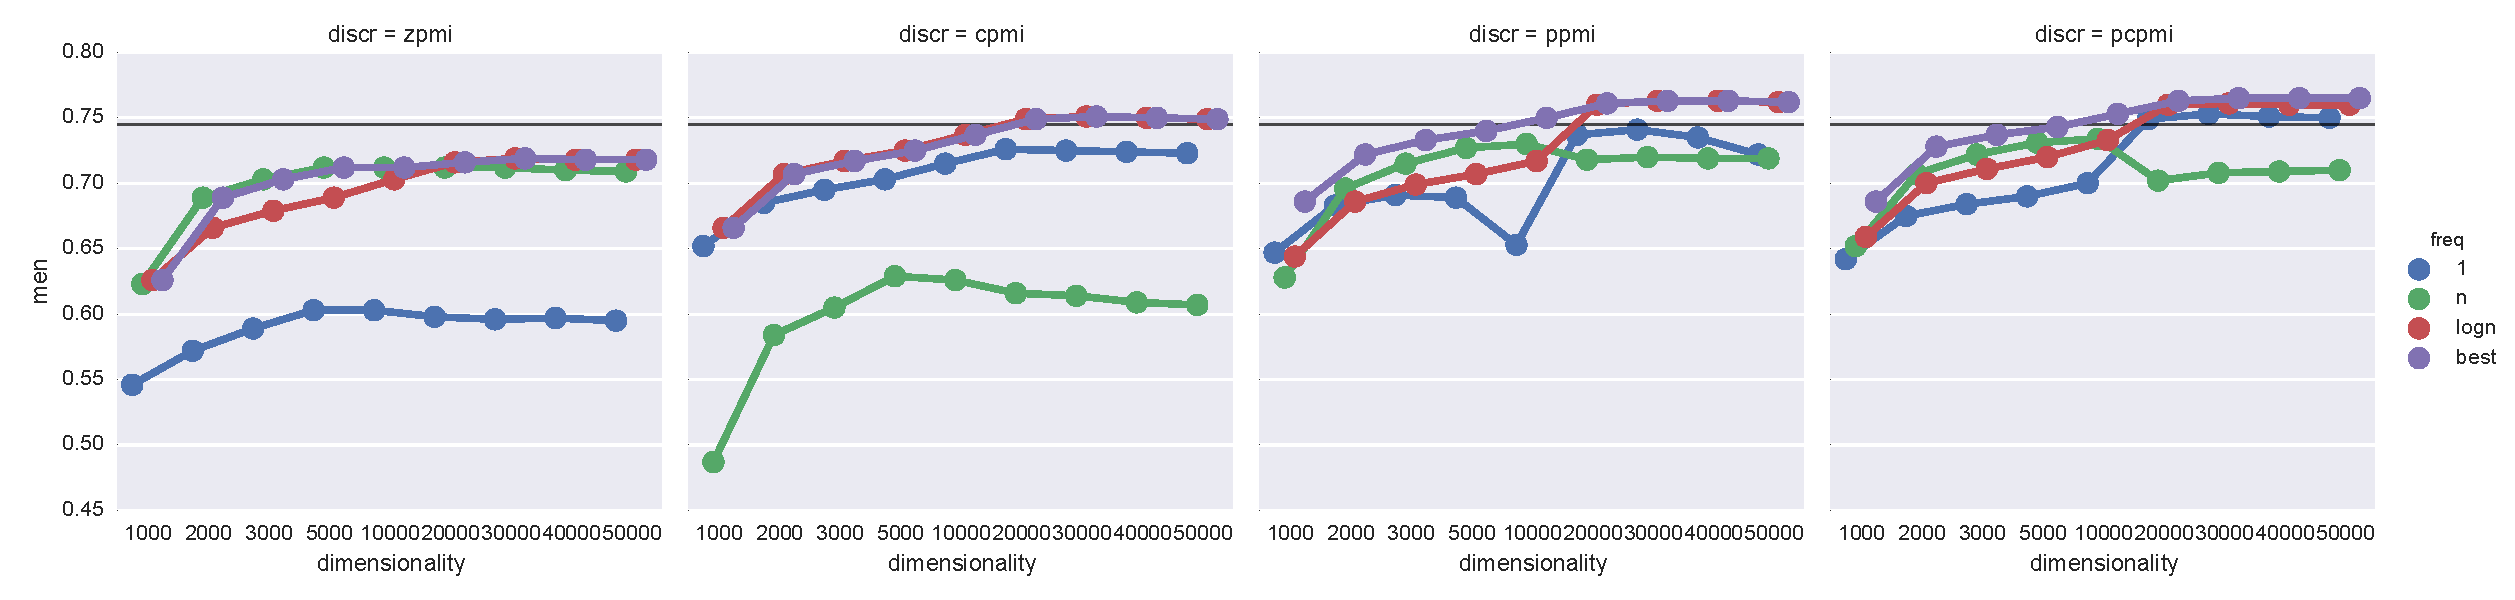
\includegraphics[width=\textwidth]{supplement/figures/men-best}
    \caption{\textbf{MEN.} The black line refers to the score of 0.745. \\
      This work: 0.765,
      SGNS: 0.774,
      GloVe: 0.729.
    }
    \label{fig:best-men}
  \end{subfigure}
  ~
  \begin{subfigure}[t]{0.37\textwidth}
    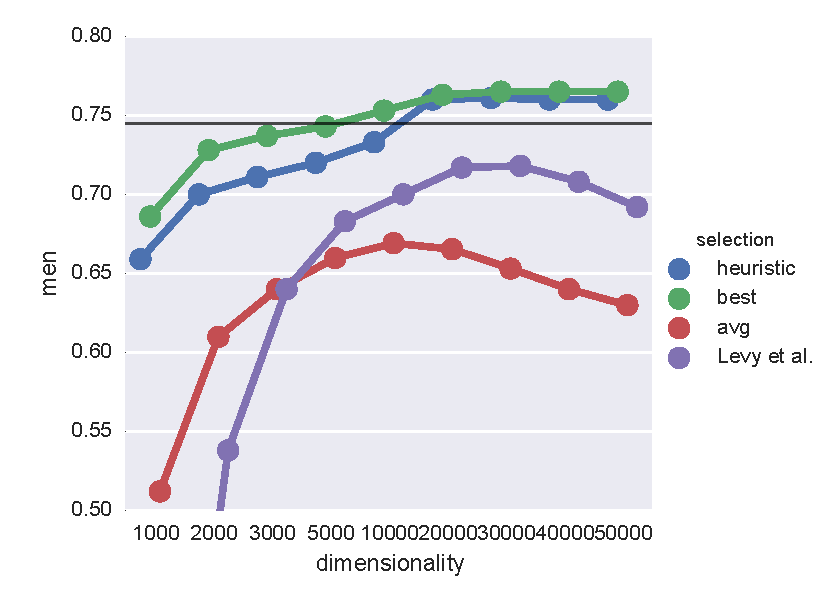
\includegraphics[width=\textwidth]{supplement/figures/men-global-best}
    \caption{\textbf{MEN.}
    }
    \label{fig:global-best-men}
  \end{subfigure}

  \caption{\textbf{Best configurations.} Black line shows the best count models reported by \protect\newcite{TACL570}. We also give our best score, SGNS and GloVe numbers from that study for comparison.}
  \label{fig:best}
\end{figure*}

%%% Local Variables:
%%% mode: latex
%%% TeX-master: "paper"
%%% End:
